\chapter{Designing the Data Capture System}
To obtain data for the Extended Kalman Filter, a data-capture system needed to be designed. Since the data sources have been identified as multiple video streams and a 9 Degrees of freedom IMU (accelerometer, gyroscope and magnetometer) the design was centred around the following equipment. The following specifications are highly modular as any camera source and any IMU with sufficient data capture rate would suffice. 

\section{GoPro Hero Session Camera}
Due to the availability of GoPro Hero Session cameras the wearable motion capture system was designed with these in mind. These cameras only take up a volume of $250cm^3$ and have a square housing measuring $6.3cm$ on all sides. The following figure presents a 3D rendered model of the camera.

\begin{figure}[!ht] 
\captionsetup{width=\linewidth, font=small}  
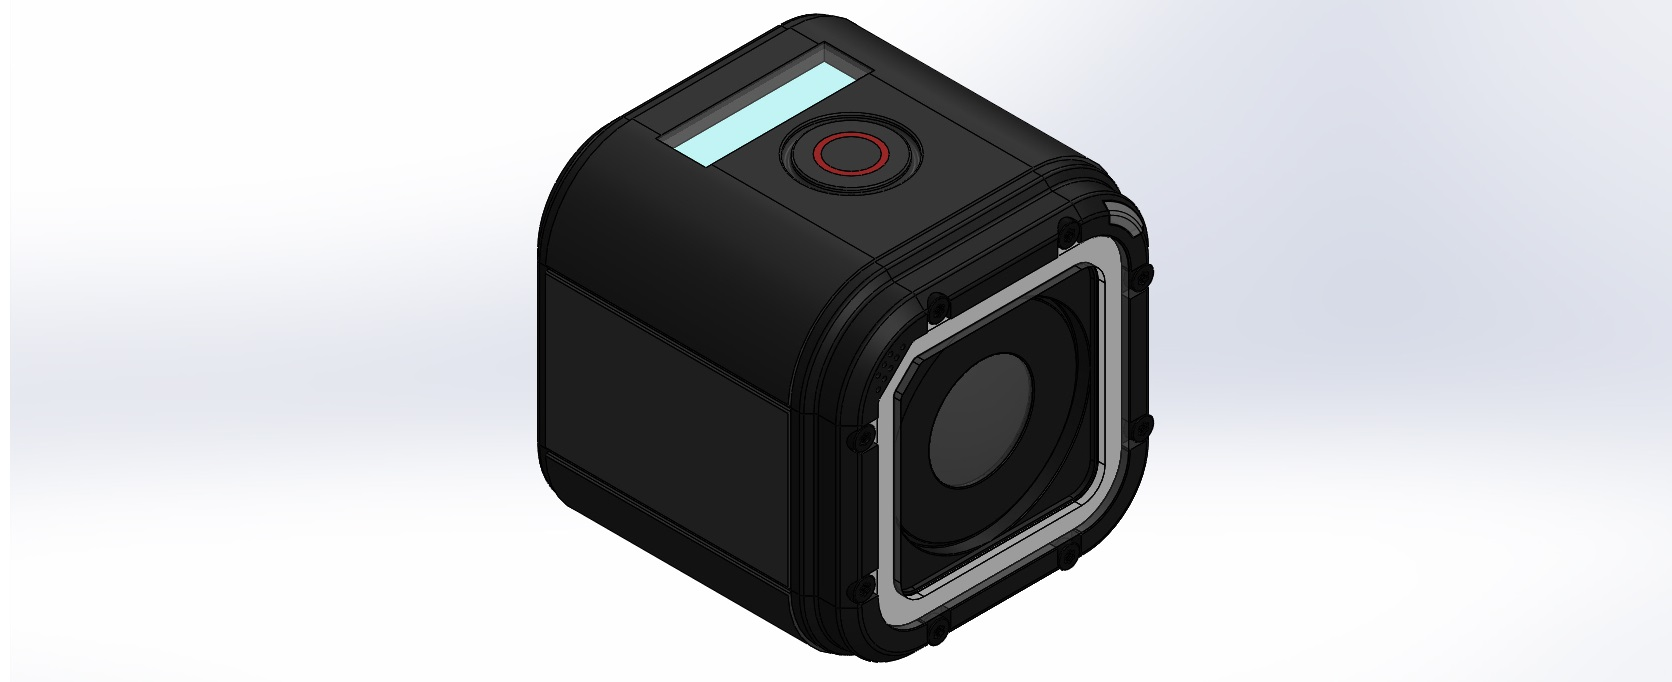
\includegraphics[width=\linewidth]{figures/GoProHero4Session.JPG}
\caption{3D CAD rendering of the GoPro Hero Session action camera}
\label{fig:GoProHero4Session}
\end{figure}

The camera can capture videos at a variety of frame rates and a variety of resolutions. These settings are limited as the software that controls the camera is proprietary. These set frame rates and resolutions are presented in the table below.

\begin{table}[!ht]
\centering
\caption{Possible frame rate and resolution combinations on the GPHS camera}
\label{framesres}
\begin{tabular}{ll}
Resolution  & Frame Rates                             \\
1920 x 1440 & 30 fps, 25 fps                          \\
1920 x 1080 & 60 fps, 50 fps, 48 fps, 30 fps, 25 fps  \\
1280 x 960  & 60 fps, 50 fps, 30 fps, 25 fps          \\
1280 x 720  & 100 fps, 60 fps, 50 fps, 30 fps, 25 fps \\
848 x 480   & 120 fps, 100 fps                       
\end{tabular}
\end{table}

The relative motion of the lower limbs appeared to move rapidly and therefore the highest possible frame rate with the best resolution was chosen. The camera was configured to record at 100Hz and at a resolution of 1280 x 720 pixels. This was chosen as the quality of the 848 x 480 video was simply to low to identify the marker centres with computer algorithms.

The camera also has the ability to record using a normal lens or a wide angle lens. The field of view of the camera greatly increases with the wide angle lens but its focal length decreases proportionally. The wide lens also produces more distortion when compared to the normal lens. Due to the relatively narrow area of capture needed the camera was configured to use the normal lens as it would decrease distortion without compromising the area of interest.

Of course working with proprietary hardware there are some difficulties. One of these difficulties is created by the GoPro camera regulating its exposure automatically. In darker environments the GoPro will automatically change to low light mode, causing inconsistent light levels in videos taken in different conditions. This introduces difficulties when trying to use feature detection since the varying light levels change the relative colors of the markers.

Another difficulty is the output video files generated by the GoPro. These files have a .MP4 file extension implying that they have already been compressed. This compression causes a loss of precision opposed to the raw video data being recorded. Compression has been implemented to save memory on the GoPro's micro SD memory card. Decompressing this video data will be discussed in the following chapter.


\section{Camera Mount Design}
Some initial work on modelling a housing for the camera was completed by the Mechatronics Lab. This was a 2 part 3D printable enclosure with no mounting points or control access. This enclosure is pictured below.

\begin{figure}[!ht] 
\captionsetup{width=0.6\linewidth, font=small}  
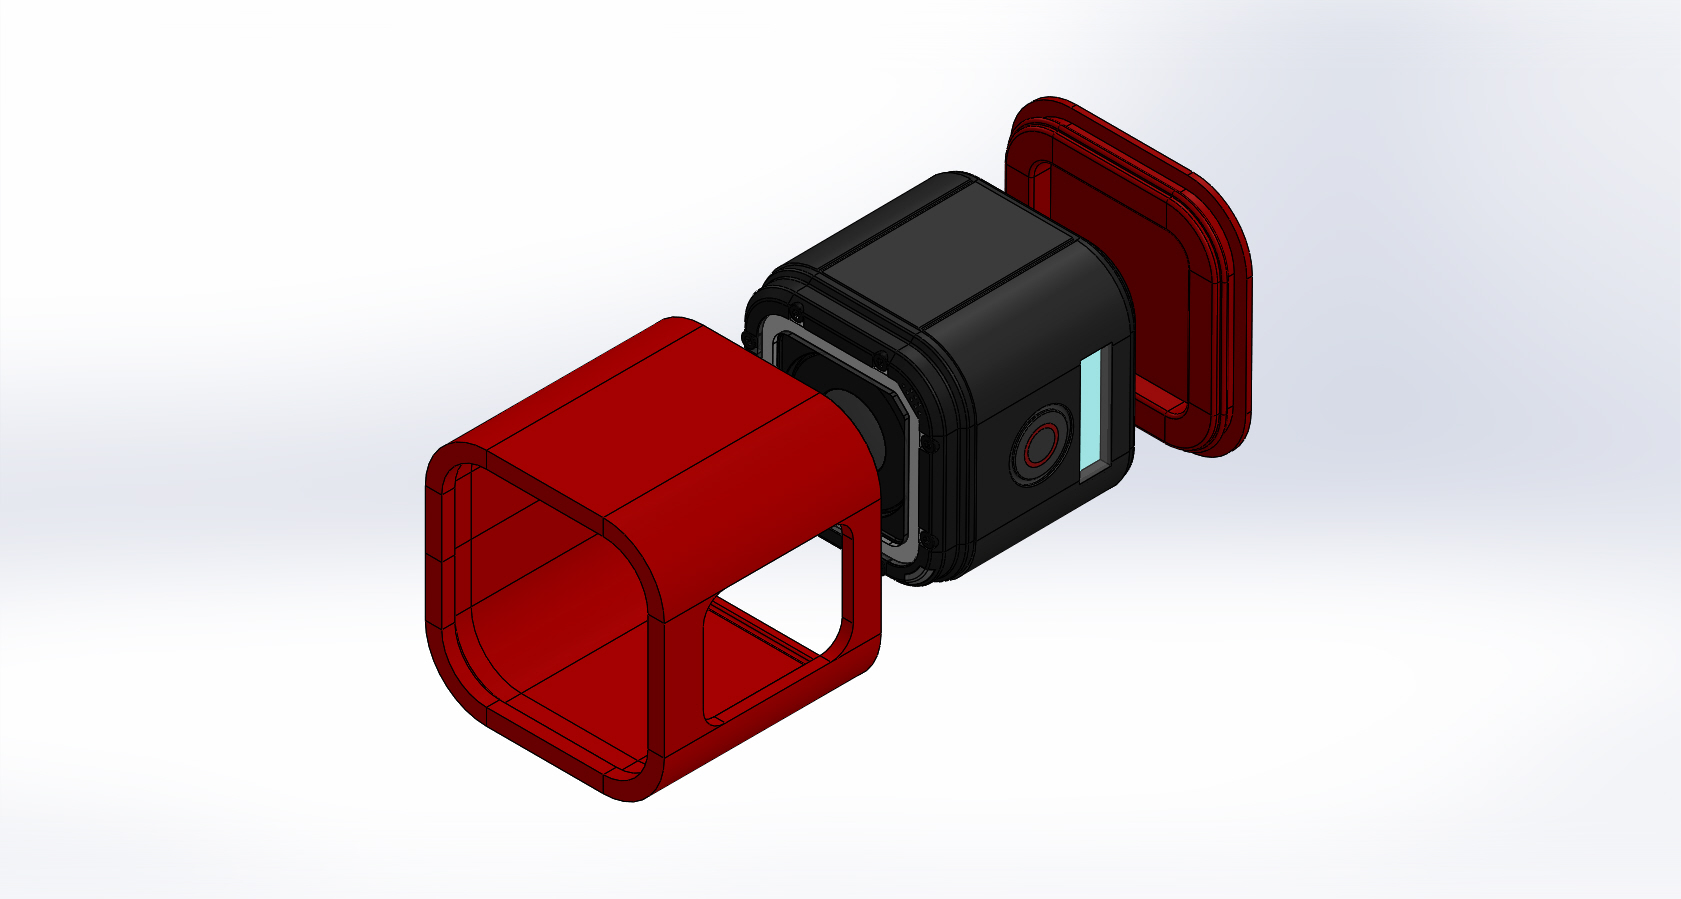
\includegraphics[width=0.6\linewidth]{figures/sylvanexploded.JPG}
\caption{Initial camera enclosure designed by the mechatronics lab}
\label{fig:sylvanexploded}
\end{figure}

This model was heavily modified using Dassault Systems SOLIDWORKS software to enclose 2 cameras mounted side by side. The bracket also needed a mounting point to join to the chest mount. Finally the bracket needed to be lightweight, provide access to the camera controls and not obscure the built in status screen of the cameras. The following figure shows the final dual camera bracket that was 3D printed. This bracket can be found on the accompanying CD.

\begin{figure}[!ht] 
\captionsetup{width=\linewidth, font=small}  
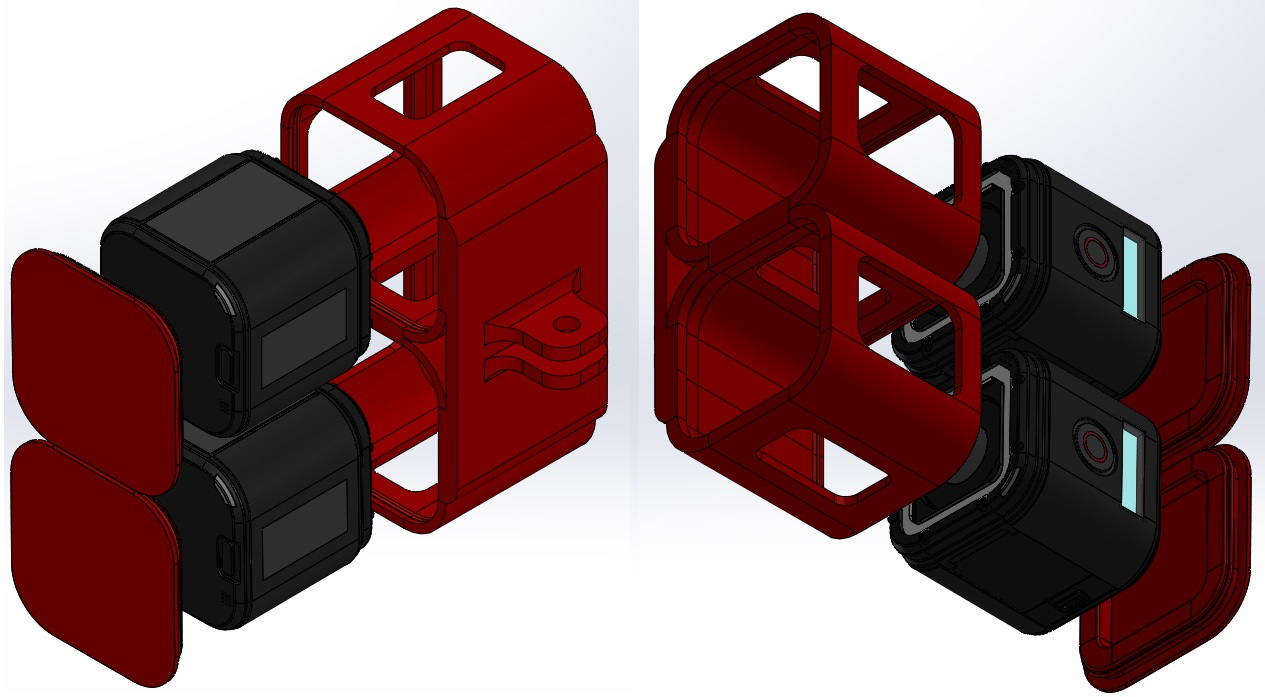
\includegraphics[width=\linewidth]{figures/stereoholder.JPG}
\caption{Final dual camera enclosure designed by the author}
\label{fig:stereoholder}
\end{figure}

This bracket was mounted to the Action Mounts Chest mount. One bracket was mounted to the front of the chest mount and using the included GoPro mounting pads the chest harness was modified to carry a bracket on the back plate as well. The back plate of the Chest Harness was relatively small and when examining the footage taken during test runs the rear camera pair was found to be very unstable. The following diagram shows the chest harness.

\begin{figure}[!ht] 
\captionsetup{width=\linewidth, font=small}  
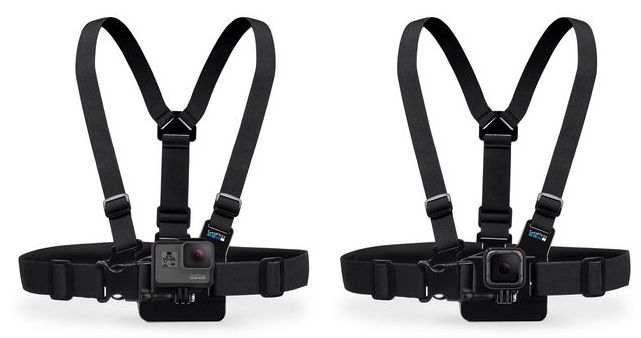
\includegraphics[width=\linewidth]{figures/chesty.png}
\caption{Action Mounts chest mount showing the fron mounting plate}
\label{fig:chesty}
\end{figure}

The need to increase the stability without hindering wearability introduced a new specification to be incorporated into the design process. The part had to comfortably fit to the back of a runner while providing a larger surface area for the camera to mount too. The part shown in the following figure was created and tested to fulfil this specification.

\begin{figure}[!ht] 
\captionsetup{width=\linewidth, font=small}  
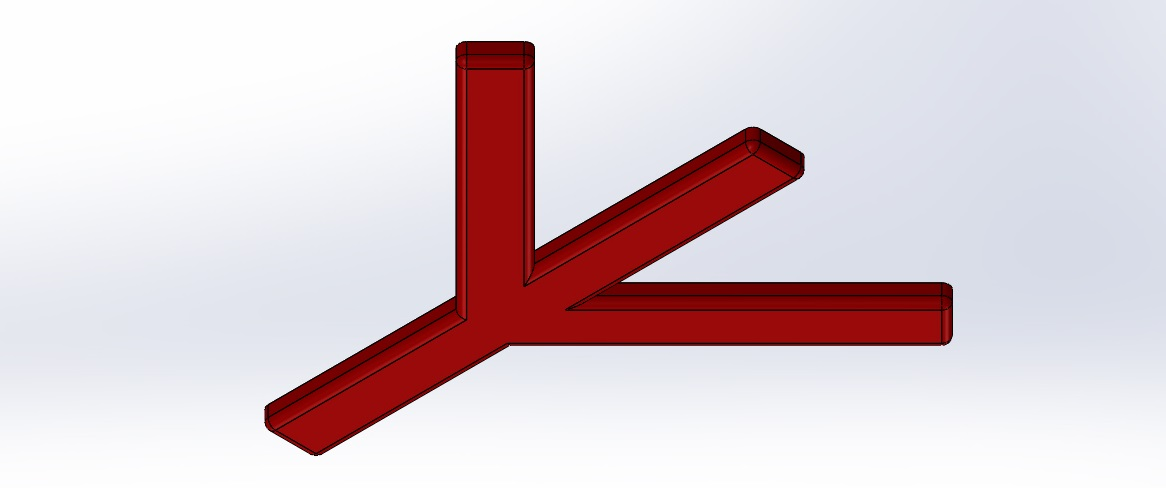
\includegraphics[width=\linewidth]{figures/stabil.JPG}
\caption{stabilizer}
\label{fig:stabil}
\end{figure}


\section{Smartphone Mount Design}
The final design specification was to rigidly mount the smart phone to the 


\section{Vision Calibration}
In order to obtain accurate positional information from the video cameras calibration was performed. MATLAB has a built in stereo camera calibration application that can calibrate a set of cameras and create an object containing all the essential parameters, including the individual camera intrinsics.

To calibrate the cameras pictures of a white and black chequerboard is fed in to the calibration application that then mathematically determines the camera parameters. In order to make this process more efficient a video of the the moving chequerboard was taken and various frames of importance extracted using a simple MATLAB script. 

\section{Smartphone Calibration}
Using the Smartphone IMU comes with several advantages and disadvantages. These disadvantages 

\section{Critical Point Markers}
To increase the accuracy of the image processing elements of this methodology various colourful markers were used to identify critical points on the subjects lower extremities. The following picture show the location of the markers.

\begin{figure}[!ht] 
\captionsetup{width=\linewidth, font=small}  
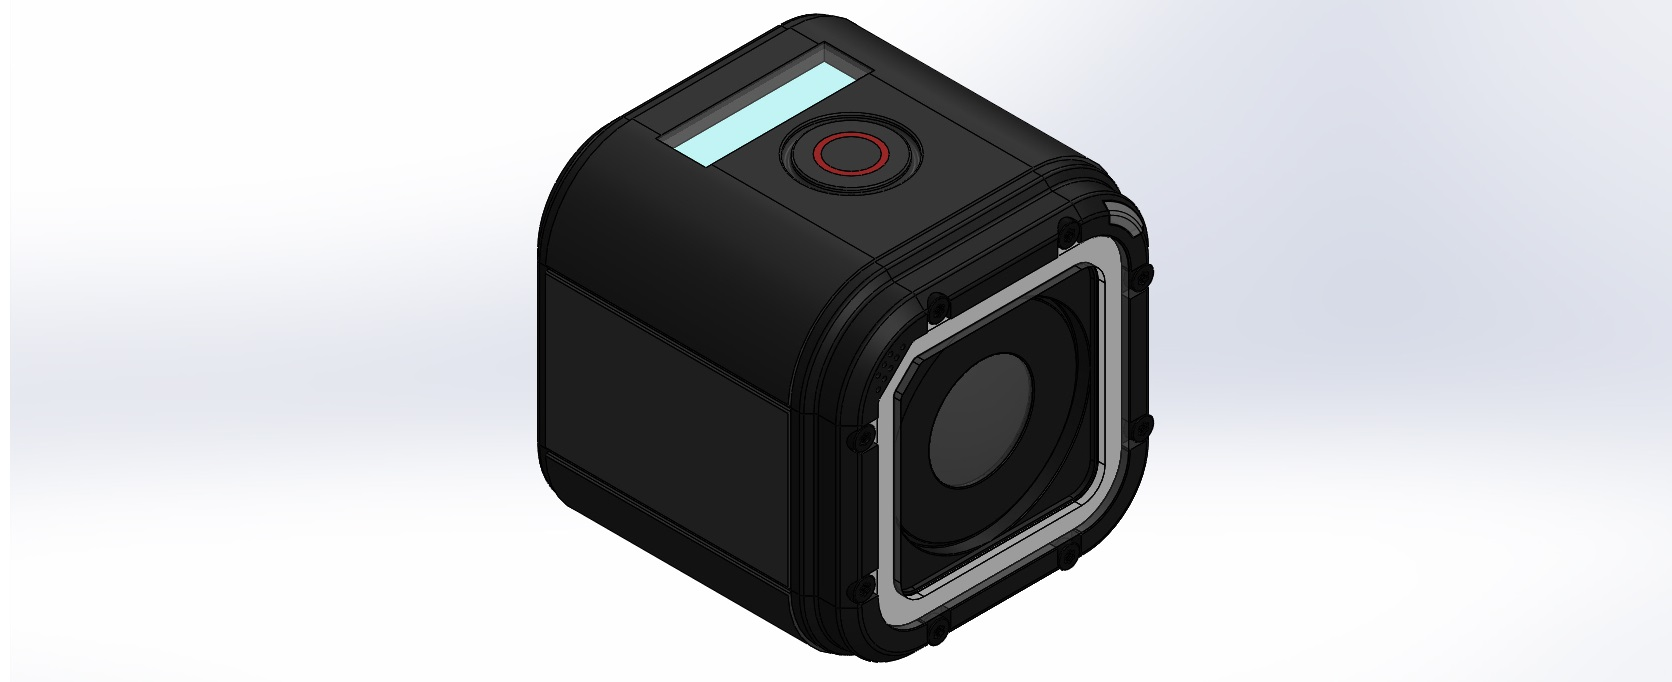
\includegraphics[width=\linewidth]{figures/GoProHero4Session.JPG}
\caption{Subject wearing Green and Pink }
\label{fig:GoProHero4Session}
\end{figure}




